\chapter{Arithmetic and Logic Unit}

\section{Overview}
We can use the following to understand the abstract implementation:

\begin{center}
  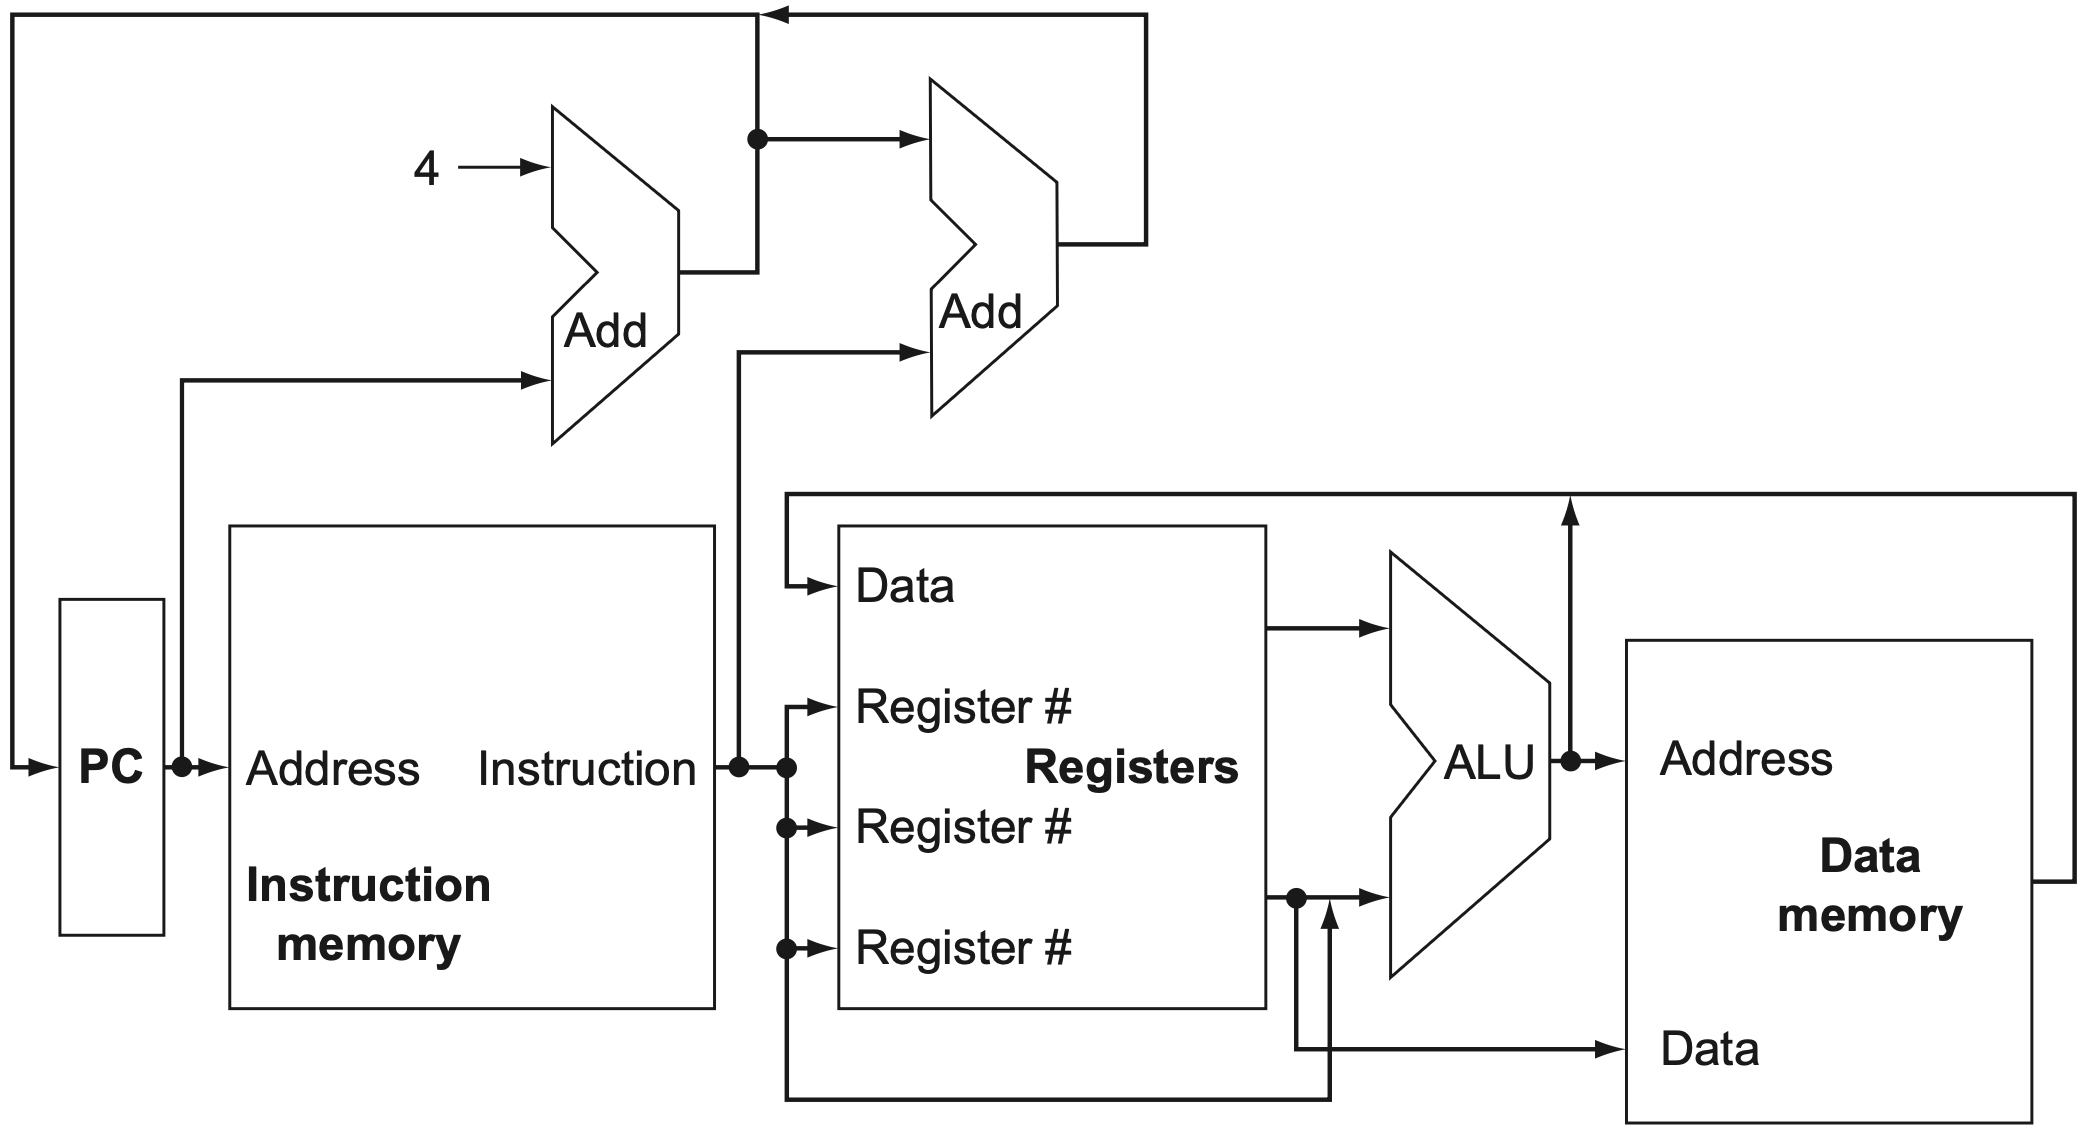
\includegraphics[width=0.8\textwidth]{Figure/AIV.png}
\end{center}

Here, the ALU (Arithmetic Logic Unit) is responsible for performing arithmetic and logical operations. It receives instructions from the registers or instruction memory.

Before we dive into this topic, we can take a look on VHDL. VHDL is a hardware description language used to model and simulate the behavior of electronic systems, particularly digital circuits. It allows designers to describe the structure and functionality of a circuit at different levels of abstraction, from the behavioral to the structural level. 

In the basic structure of VHDL, we design entity-architecture descriptions. The entity defines the system's interface, including externally visible characteristics such as ports and generic parameters. The architecture describes the system's internal behavior or structure, including internal signals and how the components interact. VHDL uses a time-based execution model to simulate and model the concurrent operations of digital systems.

For example, the assignment of A + B to result in the context of a Carry-Save Adder (CSA) would typically be part of the architecture description, as it defines the internal behavior and computation of the system.

For machine number representation, we use binary number integers. However, we need to consider storage limitations (overflow) and the representation of negative numbers.

In 32-bit signed numbers, the range is from \(2^{31} - 1\) to \(-2^{31}\). However, if the bit string represents an address, we only need to deal with unsigned integers, which range from 0 to \(2^{32} - 1\).

To perform extension, we need to consider sign extension. Sign extension copies the most significant bit into the other bits to preserve the sign of the number. For example, to extend \verb|0010|, we have \verb|0000 0010|, and for \verb|1010|, we have \verb|1111 1010|.

Then, let's take a look at some arithmetic units.

\section{Addition Unit}
To build a 1-bit binary adder, we can use the XOR gate. Here's the truth table for the 1-bit adder:

\begin{table}[H]
  \centering
  \begin{tabular}{c|c|c|c|c}
      \toprule
      A & B & Carry in & Carry out & S  \\
    \midrule
      0 & 0 & 0 & 0 & 0  \\
      0 & 0 & 1 & 0 & 1  \\
      0 & 1 & 0 & 0 & 1  \\
      0 & 1 & 1 & 1 & 0  \\
      1 & 0 & 0 & 0 & 1  \\
      1 & 0 & 1 & 1 & 0  \\
      1 & 1 & 0 & 1 & 0  \\
      1 & 1 & 1 & 1 & 1  \\
      \bottomrule
  \end{tabular}
\end{table}
Where:

- \( S = A \oplus B \oplus \text{Carry in} \)

- \( \text{Carry out} = (A \& B) | (A \& \text{Carry in}) | (B \& \text{Carry in}) \)

To build a 32-bit adder, we can connect the carry-out of the least significant bit from the previous adder to the carry-in of the next least significant bit, and connect all 32 adders in sequence. This is called the Ripple Carry Adder. However, it is slow and involves a lot of glitching.

Glitching refers to the invalid and unpredictable output that can be read by the next stage, potentially resulting in incorrect behavior. This can be interpreted as a delay, where the outputs are not stable in time to be used in the subsequent operations.

The critical path (the longest sequence of dependent operations) is \(n \times \text{CP}\), where \(n\) is the number of bits and \(CP\) is the time required for one full operation. This makes the Ripple Carry Adder slow because each bit's carry-out depends on the previous bit's carry-in, leading to a cumulative delay.

With the control unit, we can use the same structure to implement both an adder and a subtractor. 

By tailoring the ALU, we can support various instructions in the ISA, including logic operations, branch operations, and others. 

For example, after performing subtraction, we mark the result as 1 if the subtraction yields a negative result, and 0 otherwise. Then, we tie the most significant bit to the low-order bit of the input. This way, we complete a \verb|slt| operation. 

Overflow occurs when the result is too large to be represented. For example, adding two positive numbers yields a negative, adding two negative numbers gives a positive, subtracting a negative from a positive gives a negative, or subtracting a positive from a negative gives a positive. This leads to an exception. To fix this, we can modify the most significant bit to determine the overflow output setting.

\section{Multiplication and Division}

\subsection{Multiplication}
Multiplication is more complicated than addition. It can be accomplished by shifting and adding. For an \(n\)-bit \(\times\) \(m\)-bit multiplication, we must have \(n + m\) bits to cover all possible products.

The first version of multiplication needs a \(2n\)-bit adder for the multiplication of an \(n\)-bit and \(n\)-bit number, starting from the right half.
\begin{center}
  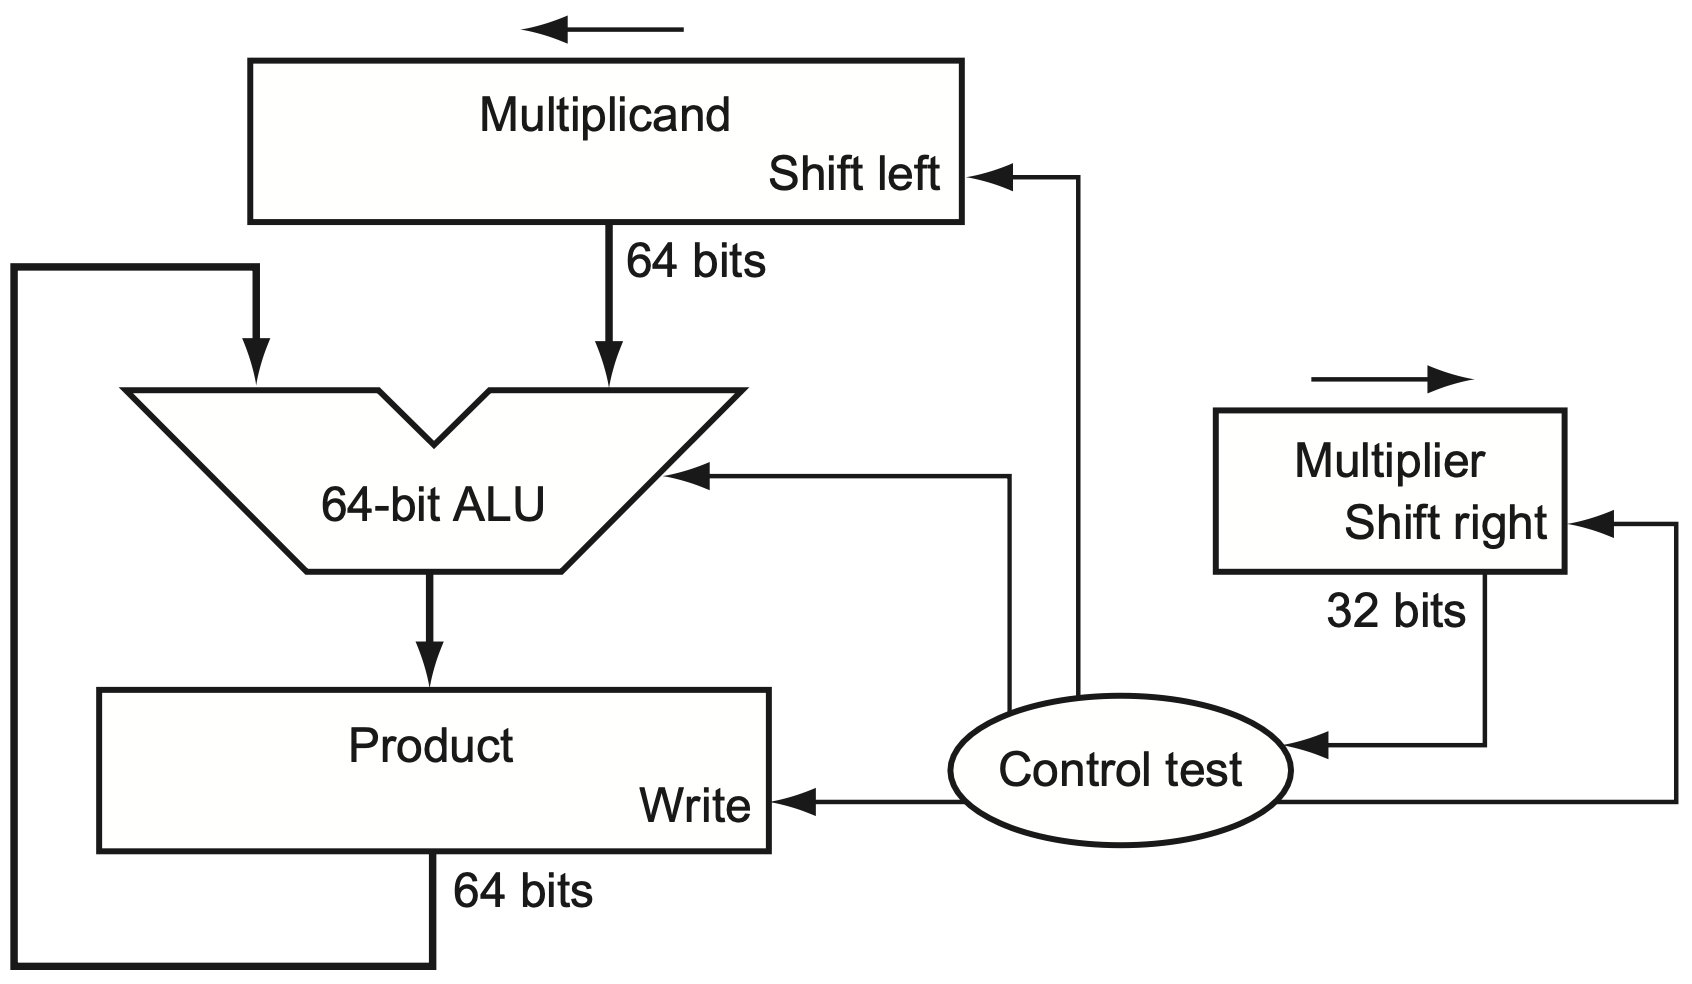
\includegraphics[width=0.5\textwidth]{Figure/mul_1.png}
\end{center}

The refined version simplifies this by requiring only an \(n\)-bit adder for the same operation.
\begin{center}
  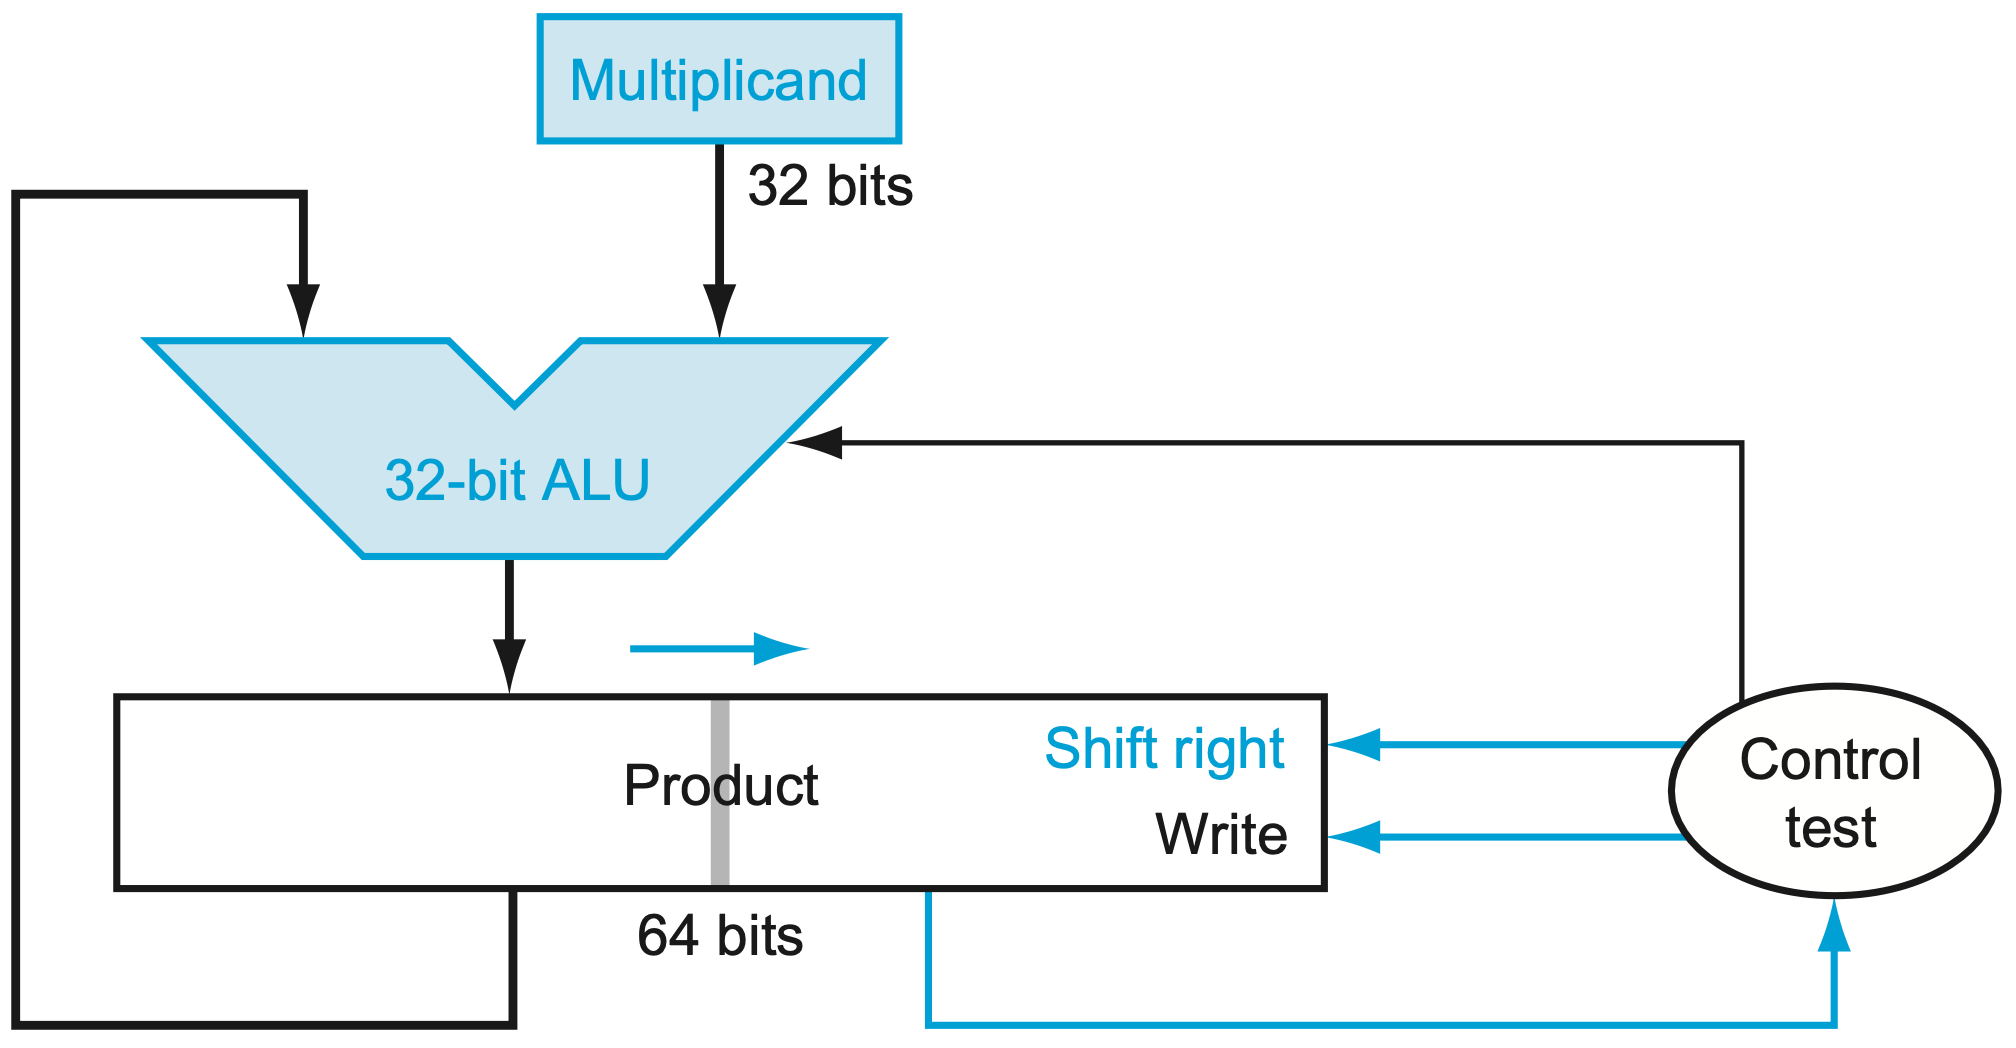
\includegraphics[width=0.5\textwidth]{Figure/mul_2.png}
\end{center}

For example, when calculating \(0010_2 \times 0011_2\), we have
\begin{table}[H]
\centering
\begin{tabular}{c|c|c|c|c}
    \hline
    \multicolumn{5}{c}{\texttt{0010} \(\times\) \texttt{0011}} \\ \hline
    Iteration & Step & Multiplier & Multiplicand & Product \\ \hline
    0 & Initial values & 001\underline{1} & 0000 0010 & 0000 0000 \\ \hline
    \multirow{3}{*}{1} & 1a: 1 \(\Rightarrow\) Prod = Prod + Mcand & 0011 & 0000 0010 & 0000 0010 \\ \cline{2-5}
      & 2: Shift left Multiplicand & 0011 & 0000 0100 & 0000 0010 \\ \cline{2-5}
      & 3: Shift right Multiplier  & 000\underline{1} & 0000 0100 & 0000 0010 \\ \hline
    \multirow{3}{*}{2} & 1a: 1 \(\Rightarrow\) Prod = Prod + Mcand & 0001 & 0000 0100 & 0000 0110 \\ \cline{2-5}
      & 2: Shift left Multiplicand & 0001 & 0000 1000 & 0000 0110 \\ \cline{2-5}
      & 3: Shift right Multiplier  & 000\underline{0} & 0000 1000 & 0000 0110 \\ \hline
    \multirow{3}{*}{3} & 1: 0 \(\Rightarrow\) No operation & 0000 & 0000 1000 & 0000 0110 \\ \cline{2-5}
      & 2: Shift left Multiplicand & 0000 & 0001 0000 & 0000 0110 \\ \cline{2-5}
      & 3: Shift right Multiplier  & 000\underline{0} & 0001 0000 & 0000 0110 \\ \hline
    \multirow{3}{*}{4} & 1: 0 \(\Rightarrow\) No operation & 0000 & 0001 0000 & 0000 0110 \\ \cline{2-5}
      & 2: Shift left Multiplicand & 0000 & 0010 0000 & 0000 0110 \\ \cline{2-5}
      & 3: Shift right Multiplier  & 000\underline{0} & 0010 0000 & 0000 0110 \\ \hline
\end{tabular}
\end{table}

\verb|mul| performs a 32-bit \(\times\) 32-bit multiplication and places the lower 32 bits in the destination register. \verb|mulh|, \verb|mulhu|, and \verb|mulhsu| perform the same multiplication but return the upper 32 bits of the full 64-bit product.

\subsection{Division}
Division is just a series of quotient digit guesses, left shifts, and subtractions.

In the first version of division, the 32-bit divisor starts in the left half of the divisor register and is shifted right 1 bit each iteration.
\begin{center}
  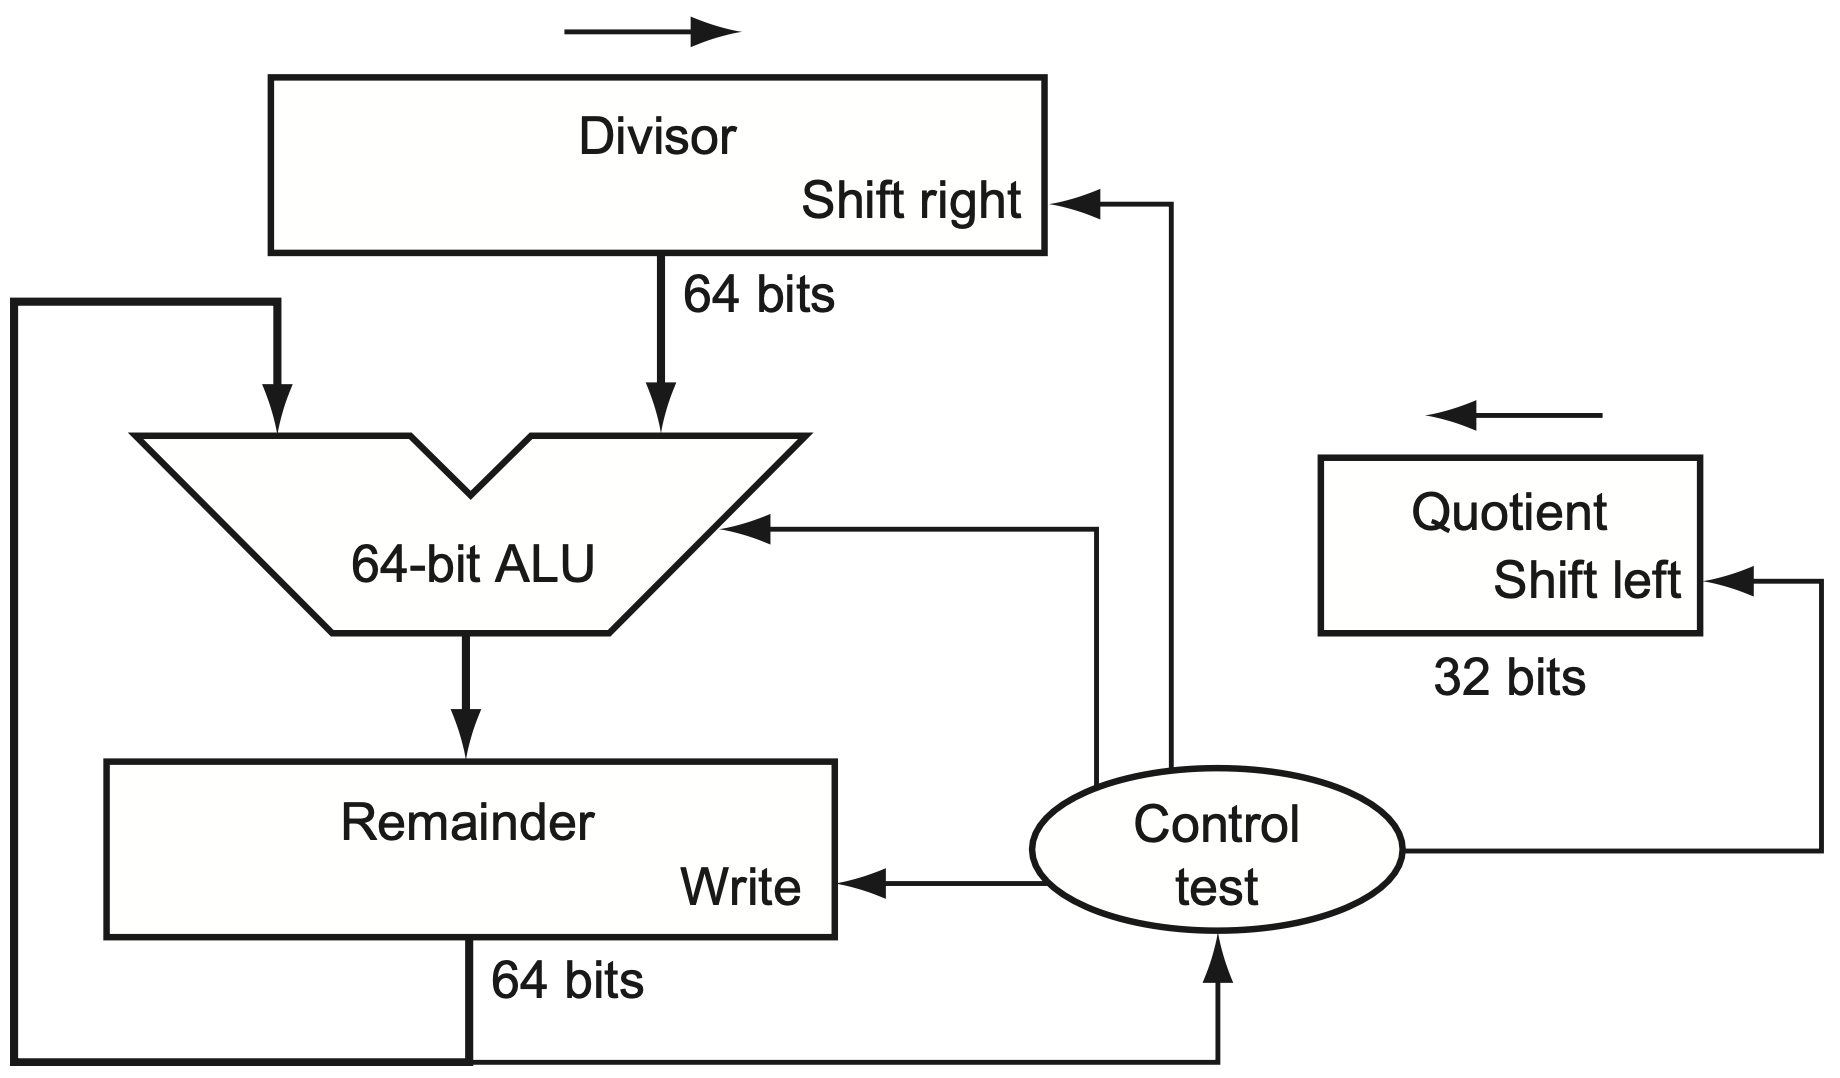
\includegraphics[width=0.5\textwidth]{Figure/div_1.png}
\end{center}

The refined version combines the Quotient register with the right half of the Remainder register.
\begin{center}
  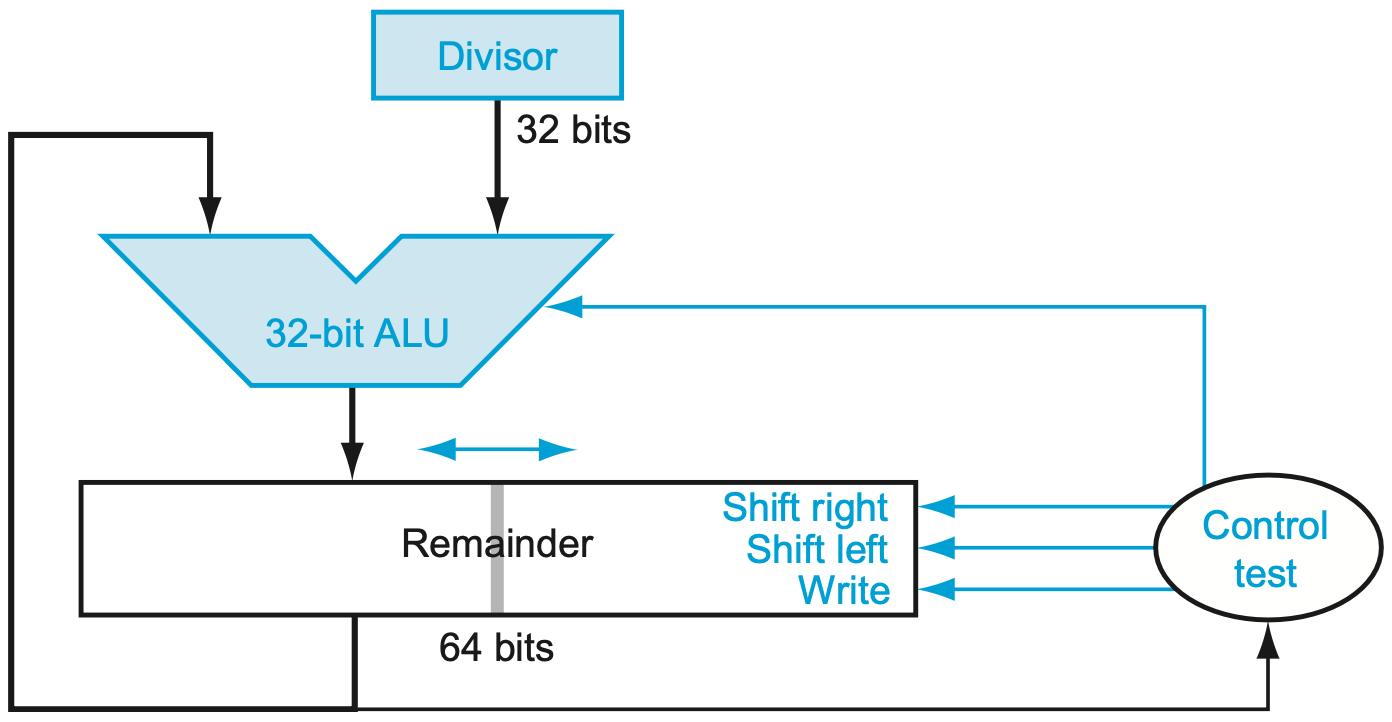
\includegraphics[width=0.5\textwidth]{Figure/div_2.png}
\end{center}

\verb|div| generates the remainder in \verb|hi| and the quotient in \verb|lo|. It performs a 32-bit by 32-bit signed integer division of \verb|rs1| by \verb|rs2|, rounding towards zero. \verb|div| and \verb|divu| perform signed and unsigned integer division of 32 bits by 32 bits. \verb|rem| and \verb|remu| provide the remainder of the corresponding division operation.

\section{Shifter}
Shifts by a constant are encoded as a specialization of the I-type format. The operand to be shifted is in rs1, and the shift amount is encoded in the lower 5 bits of the I-immediate field.
\begin{codeBlock}
  srli rd, rs1, imm[4:0]
  srai rd, rs1, imm[4:0]
\end{codeBlock}

\verb|slli| is a logical left shift, \verb|srli| is a logical right shift, and \verb|srai| is an arithmetic right shift. Logical shifts fill with zeros, while arithmetic right shifts fill with the sign bit. For example, a logical right shift of \verb|1111| by 2 bits results in \verb|0011|, while an arithmetic right shift of \verb|1111| by 2 bits results in \verb|1111|. 

A simple shifter can be accomplished by using a series of multiplexers to shift the input data by a specified number of bit positions, either left or right.
\begin{center}
  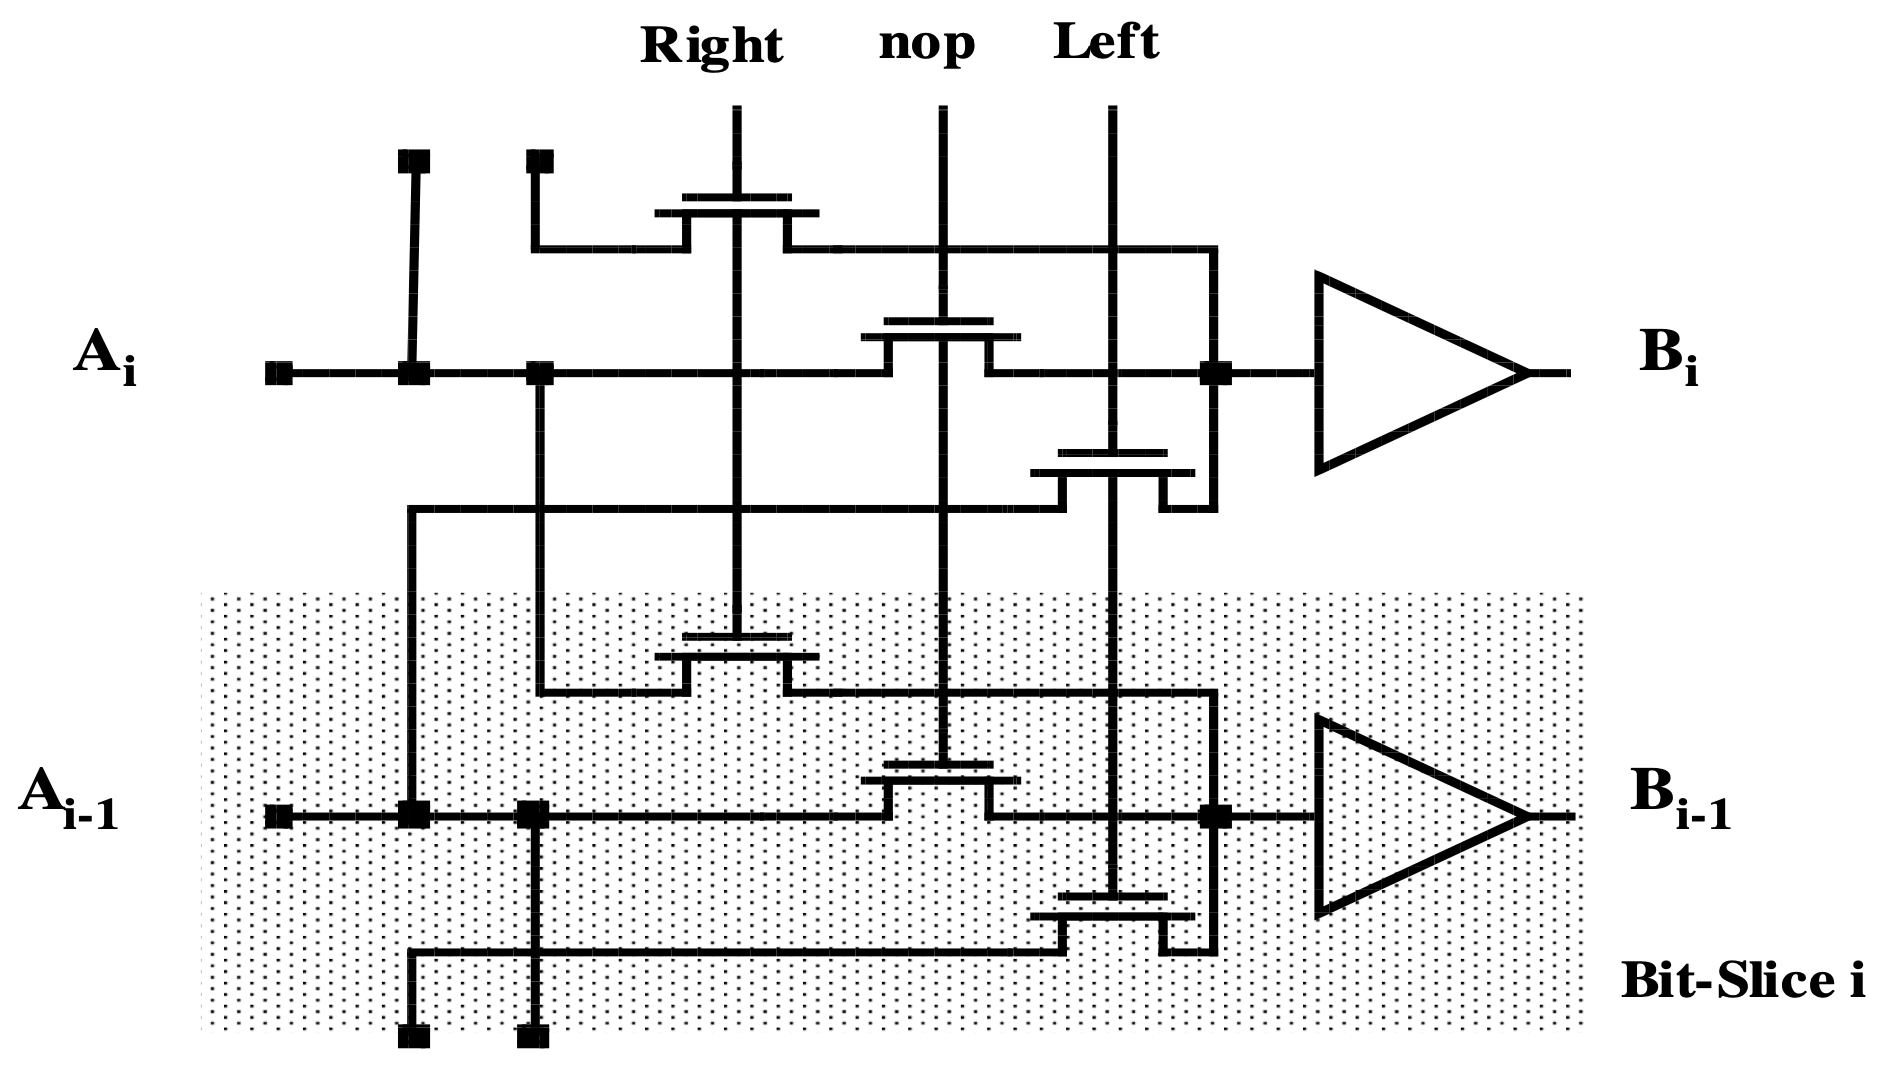
\includegraphics[width=0.5\textwidth]{Figure/shifter_1.png}
\end{center}

For example, to do a right shift, let Right = 1 and nop = Left = 0. Then, \(B_{i-1} = A_i\), where \(B\) is the shifted output and \(A\) is the input. 

In a parallel programmable shifter, we can use control signals to decide the shift amount, direction, and type. The control logic determines how many positions the data should be shifted, whether it should be shifted left or right, and whether the shift should be logical or arithmetic. This allows for flexible shifting operations based on the input values and the specified parameters.

A logarithmic shifter is a more complex shifter that can perform shifts based on logarithmic scaling. It involves specialized shifting mechanisms used for fast multiplication and division by powers of 2. With one shifter, we can perform a shift by 0 or 1 bit; with two shifters, we can perform shifts by 0, 1, 2, or 3 bits, and so on.